% =====================================================================
%  Predicting clogging from the contact network: a graph neural network
%  for deformable-particle suspensions at a microfluidic constriction.
%
%  Tailored for Physica A: Statistical Mechanics and its Applications.
%  Built with the generic article class so it compiles with any TeX
%  distribution. For submission, swap the header for Elsevier's
%  elsarticle class (see README.md).
%
%  Build:  pdflatex main && bibtex main && pdflatex main && pdflatex main
% =====================================================================

\documentclass[11pt,a4paper]{article}

\usepackage[T1]{fontenc}
\usepackage[utf8]{inputenc}
\IfFileExists{lmodern.sty}{\usepackage{lmodern}}{}
\usepackage[english]{babel}
\usepackage[a4paper,margin=2.4cm]{geometry}
\usepackage{amsmath,amssymb,amsfonts}
\usepackage{graphicx}
\usepackage{booktabs}
\usepackage{xcolor}
\usepackage[colorlinks=true,linkcolor=blue!50!black,
            citecolor=blue!50!black,urlcolor=blue!50!black]{hyperref}
\usepackage{caption}
\captionsetup{font=small,labelfont=bf,labelsep=period}
\usepackage{authblk}

\graphicspath{{figures/}}

\usepackage[numbers,sort&compress]{natbib}
% Use Elsevier's elsarticle-num style if available (for Physica A submission),
% otherwise fall back to plainnat. Exactly one \bibliographystyle is emitted.
\IfFileExists{elsarticle-num.bst}
  {\bibliographystyle{elsarticle-num}}
  {\bibliographystyle{plainnat}}

\title{\textbf{Predicting clogging from the contact network:
a graph neural network for deformable-particle suspensions
at a microfluidic constriction}}

\author[1]{Ram Chand\thanks{Corresponding author:
   \texttt{ram.chand@bnbwu.edu.pk}}}
\affil[1]{Department of Natural Sciences,
   The Begum Nusrat Bhutto Women University, Sukkur, Sindh, Pakistan}

\date{\today}

\begin{document}
\maketitle

% ---------------------------------------------------------------------
\begin{abstract}
\noindent When a suspension of soft particles is driven through a
narrow gap, it either flows or it jams: a load-bearing arch can form
across the constriction and arrest the flow. This clogging transition
governs everything from coffee filters and household drains to grain
hoppers and the obstruction of small blood vessels, yet most of what we
know about it comes from rigid particles and from after-the-fact
description rather than prediction. Here we ask a different question:
given a single snapshot of which particles are touching which, can one
predict whether the suspension will clog --- without integrating the
dynamics forward? We address it with a two-dimensional
lattice-Boltzmann immersed-boundary model of deformable capsules pushed
through a rectangular neck, run across ten aperture ratios spanning the
flowing and clogged regimes. Each simulation frame is converted into a
graph in which capsules are nodes and near-contacts are edges carrying
the local gap and approach rate, and an edge-aware graph neural network
is trained to classify the configuration as clogging or flowing. The
simulations reproduce the expected arching threshold near an
aperture-to-particle ratio $D/d\approx 3$. The classifier reaches an
area under the ROC curve of $0.93$ on held-out frames, and --- under a
leave-one-run-out test that removes all correlation between training
and test configurations --- it generalises to runs it has never seen
with a mean accuracy of $0.87$, failing only at the single aperture
sitting exactly on the transition, where the outcome is genuinely
ambiguous. The result shows that the instantaneous contact network
carries a learnable, transferable signature of imminent clogging in
deformable suspensions, and it provides a reproducible pipeline from
mesoscale simulation to graph-based prediction.

\vspace{1em}
\noindent\textbf{Keywords:}
clogging~\textperiodcentered~jamming~\textperiodcentered~
soft-particle suspensions~\textperiodcentered~contact network~
\textperiodcentered~graph neural network~\textperiodcentered~
lattice Boltzmann method~\textperiodcentered~immersed boundary method
\end{abstract}

% ---------------------------------------------------------------------
\section{Introduction}
\label{sec:intro}

Push a crowd of particles through an opening only a few particle
diameters wide and one of two things happens. Either the particles file
through and the flow continues, or a handful of them lock into a stable
arch that spans the opening and brings the flow to a halt. This
clogging, or jamming at a bottleneck, is one of the most familiar
failure modes in nature and technology: it is why coffee grounds bridge
a filter, why a kitchen drain blocks with debris, why grain stalls in a
silo, and why circulating cells and particulates can obstruct a narrow
vessel. It is also a long-standing problem in the statistical physics of
disordered and athermal systems, because the arch is a collective,
force-bearing structure that forms intermittently and is sensitive to
the microscopic arrangement of contacts~\citep{dressaire2017clogging,
marin2025clogging}.

A large body of experimental and computational work has mapped when
clogging occurs. For rigid grains and hard spheres flowing through a
constriction, the controlling quantity is the ratio of the aperture
width to the particle diameter: permanent clogs form below an
aperture-to-particle ratio of roughly two to four, where a small number
of particles can bridge the gap, while wider openings sustain
continuous or intermittent flow~\citep{marin2018clogging,
souzy2020transition}. Softness changes the picture. Deformable particles
can squeeze through gaps that would arrest rigid ones, so the clogging
boundary shifts and the dynamics of the arch differ from the granular
case~\citep{hong2017clogging, bielinski2021squeezing}. Most of this
literature, however, is descriptive: it characterises the statistics of
clogging events, the arch lifetimes, and the dependence on geometry and
volume fraction. Comparatively little of it is \emph{predictive} at the
level of an individual configuration, and almost none of it treats the
clog as a property of the contact network that could be read off
directly.

Machine learning on graphs offers a natural language for that question.
A suspension at an instant in time is, after all, a graph: the particles
are nodes and their mechanical contacts are edges. Graph neural networks
(GNNs) learn functions on exactly this kind of irregular, relational
data by passing messages along edges~\citep{gilmer2017neural,
kipf2017semi, hamilton2017inductive}, and they have recently been used as
fast surrogates for the \emph{dynamics} of particulate suspensions, for
example by learning the hydrodynamic mobility of a configuration so that
its motion can be integrated cheaply~\citep{ma2022fast}. Those efforts
target rigid particles and the forward problem of time evolution. The
complementary question --- whether a GNN can read the contact network of
a \emph{deformable} suspension and predict a collective outcome such as
clogging, without any time integration at all --- has not, to our
knowledge, been addressed.

That is the question of this paper. We build a two-dimensional
lattice-Boltzmann immersed-boundary (LBM--IBM) model of soft capsules
driven through a rectangular constriction, run it across a range of
aperture ratios that brackets the flowing and clogged regimes, and from
the resulting trajectories extract, for every saved frame, the contact
graph of the suspension. We then train an edge-aware GNN to classify
each graph as belonging to a clogging or a flowing run, and we evaluate
it honestly: not only on randomly held-out frames, but with a
leave-one-run-out protocol in which an entire aperture is removed from
training, so that the test configurations are statistically independent
of those the network has seen. The simulations reproduce the expected
arching threshold near $D/d\approx 3$; the classifier attains an area
under the ROC curve of $0.93$ on held-out frames and a leave-one-run-out
accuracy of $0.87$, with its only weakness lying exactly at the
aperture on the transition. The contribution is twofold: a demonstration
that the instantaneous contact network carries a learnable and
transferable signature of clogging in soft suspensions, and a
reproducible pipeline that connects a mesoscale physics solver to a
graph-based predictor.

The remainder of the paper is organised as follows.
Section~\ref{sec:methods} sets out the fluid solver, the capsule and
contact models, the geometry and driving, the clogging diagnostic, the
graph construction, and the network and its training.
Section~\ref{sec:results} reports the clogging transition, the
classifier performance, the leave-one-run-out generalisation, and the
structural difference between the regimes. Section~\ref{sec:discussion} interprets
the findings, reports a negative result on data augmentation, and states
the limitations. Section~\ref{sec:conclusion} concludes.

% ---------------------------------------------------------------------
\section{Model and methods}
\label{sec:methods}

The simulations use an in-house C++ solver that couples a
lattice-Boltzmann fluid to immersed deformable capsules; all quantities
below are in lattice units (LU). Sections~\ref{sec:lbm}--\ref{sec:driving}
describe the physics, Section~\ref{sec:clogmetric} the clogging
diagnostic, and Sections~\ref{sec:graph}--\ref{sec:training} the graph
representation and the neural network.

\subsection{Lattice-Boltzmann fluid}
\label{sec:lbm}

The fluid is solved on a regular two-dimensional grid with the D2Q9
velocity set $\{\boldsymbol e_i\}_{i=0}^{8}$, weights $w_0=4/9$,
$w_{1\text{--}4}=1/9$, $w_{5\text{--}8}=1/36$, and lattice sound speed
$c_s^2=1/3$~\citep{kruger2017lattice}. Let $f_i(\boldsymbol x,t)$ be the
discrete distribution in direction $i$. The density and momentum are
\begin{equation}
\rho=\sum_i f_i, \qquad
\rho\,\boldsymbol u=\sum_i f_i\,\boldsymbol e_i+\tfrac{1}{2}\boldsymbol F\,\Delta t,
\label{eq:moments}
\end{equation}
and the equilibrium is the second-order Hermite truncation of the
Maxwellian,
\begin{equation}
f_i^{\mathrm{eq}}=w_i\rho\Big[1
+\frac{\boldsymbol e_i\!\cdot\!\boldsymbol u}{c_s^2}
+\frac{(\boldsymbol e_i\!\cdot\!\boldsymbol u)^2}{2c_s^4}
-\frac{\boldsymbol u\!\cdot\!\boldsymbol u}{2c_s^2}\Big].
\label{eq:feq}
\end{equation}
We evolve $f_i$ by a single-relaxation-time (BGK) collide-and-stream
step with a regularisation of the non-equilibrium part to suppress
ghost modes~\citep{latt2006lattice},
\begin{equation}
f_i(\boldsymbol x+\boldsymbol e_i\Delta t,\,t+\Delta t)
=f_i(\boldsymbol x,t)
-\frac{1}{\tau}\big[f_i-f_i^{\mathrm{eq}}\big]
+F_i\,\Delta t,
\label{eq:bgk}
\end{equation}
with relaxation time $\tau$ fixing the kinematic viscosity through
$\nu=c_s^2(\tau-\tfrac12)\Delta t$. We use $\tau=0.9$, i.e.
$\nu=0.133$~LU. A body force $\boldsymbol F=(F_x,0)$ drives the flow and
enters the collision through the second-order forcing of Guo et
al.~\citep{guo2002discrete},
\begin{equation}
F_i=\Big(1-\frac{1}{2\tau}\Big)w_i
\Big[\frac{\boldsymbol e_i-\boldsymbol u}{c_s^2}
+\frac{(\boldsymbol e_i\!\cdot\!\boldsymbol u)\,\boldsymbol e_i}{c_s^4}\Big]
\!\cdot\!\boldsymbol F .
\label{eq:guo}
\end{equation}
No-slip walls at the top and bottom of the channel are imposed by
halfway bounce-back; the streamwise direction is periodic, so the
suspension recirculates and maintains its concentration. The channel is
$N_x\times N_y=220\times 48$~LU. The driving $F_x=2.24\times10^{-5}$ was
calibrated to give a developed centre-line speed
$u_{\max}\approx 8\times10^{-3}$~LU, so that the Reynolds number
$\mathrm{Re}=u_{\max}r/\nu\approx 0.24$ and the Mach number
$u_{\max}/c_s\approx 0.014$ both sit well inside the incompressible,
Stokes-like regime appropriate to microfluidic flow.

\subsection{Immersed deformable capsules}
\label{sec:capsules}

Each capsule is a closed loop of $N_n=16$ Lagrangian nodes
$\boldsymbol X_\ell$ enclosing fluid, with rest diameter $d=8$~LU
(radius $r=4$). Two-way coupling to the fluid uses the immersed-boundary
method~\citep{peskin2002immersed}: membrane forces are spread to the
lattice and the node velocities are interpolated back, both with the
four-point Peskin regularised delta $\delta_h$,
\begin{equation}
\boldsymbol f(\boldsymbol x)=\sum_\ell
\boldsymbol F_\ell\,\delta_h(\boldsymbol x-\boldsymbol X_\ell)\,\Delta s_\ell,
\qquad
\dot{\boldsymbol X}_\ell=\sum_{\boldsymbol x}
\boldsymbol u(\boldsymbol x)\,\delta_h(\boldsymbol x-\boldsymbol X_\ell)\,\Delta x^2 .
\label{eq:ibm}
\end{equation}
The spreading--interpolation cycle is iterated $K=2$ times per step
(multi-direct forcing) to reduce the residual slip at the membrane. The
membrane resists shear and area change through a Skalak constitutive
law~\citep{skalak1973strain} with shear modulus $G_s$ and area modulus
$C=10\,G_s$, plus discrete bending ($k_b=0.02$), area ($k_a=1.0$) and
perimeter ($k_p=0.1$) penalties. The capsule deformability is set by the
capillary number $\mathrm{Ca}=\rho\,\nu\,r\,\dot\gamma/G_s$ with the wall
shear rate $\dot\gamma=4u_{\max}/N_y$; we fix $\mathrm{Ca}=0.01$ for all
runs, which fixes $G_s$ given the flow.

Two capsules (or a capsule and a wall or obstacle) interact through a
short-range repulsion that prevents membrane interpenetration. Between
nodes $a$ and $b$ at separation $r_{ab}$ below a cut-off $r_c$ the force
along the unit normal $\hat{\boldsymbol n}_{ab}$ is
\begin{equation}
\boldsymbol F^{\mathrm{rep}}_{ab}
=\epsilon\Big(\frac{\sigma}{r_{ab}}\Big)^{p}\hat{\boldsymbol n}_{ab},
\qquad r_{ab}<r_c,
\label{eq:repulsion}
\end{equation}
with $\epsilon=10^{-3}$, $\sigma=1$, $p=4$, $r_c=2$~LU. Near-contact
hydrodynamics below the grid resolution is captured by a lubrication
correction applied when the surface gap falls below $1.5$~LU. (The
solver also supports an optional dissipative-frictional contact, but it
is disabled here so that the contacts are governed by the conservative
repulsion alone.)

\subsection{Geometry, seeding and driving}
\label{sec:driving}

The constriction is a pair of rectangular obstacles spanning
$x\in[150,175]$, one growing from each wall, leaving a centred gap of
width $D=(D/d)\,d$. The single control parameter is the
aperture-to-particle ratio $D/d$. Upstream of the neck, a dense plug of
capsules is seeded in the region $x\in[40,145]$, $y\in[8,40]$ on a
hexagonal grid whose spacing $2r+\delta_{\min}$ guarantees a minimum
surface gap $\delta_{\min}=1$~LU by construction; this deterministic
``fill'' seeding reliably packs $\approx 40$ capsules, where rejection-
based random seeding leaves the region sparse. The body force then
drives the plug toward and through the neck, and because the channel is
periodic the capsules recirculate, so the system sustains a roughly
constant concentration at the constriction rather than draining.

Each run is initialised, ramped over a $2000$-step warm-up, and then
integrated for $10^4$ production steps with the capsule trajectory
written every $200$ steps. We sweep ten apertures,
$D/d\in\{1.5,2.0,2.5,2.75,3.0,3.25,3.5,4.0,4.5,5.0\}$, at fixed
$\mathrm{Ca}=0.01$, spanning the clogged and flowing regimes with
extra sampling near the transition.

\subsection{Clogging diagnostic}
\label{sec:clogmetric}

For each capsule we record the first time its centroid crosses the neck
centre $x_{\mathrm{neck}}=162.5$, and define the escaped fraction
$\eta(t)$ as the cumulative number of capsules that have crossed,
divided by the total. A run is labelled \emph{clogged} when, at the end
of the run, $\eta<0.9$ and the escape flux has stalled (no new crossing
over the final window) while capsules remain upstream; otherwise it is
\emph{flowing}. As a structural diagnostic we also compute the neck
contact number $Z$, the mean number of contacting neighbours per capsule
within a band $|x-x_{\mathrm{neck}}|\le 15$~LU, where a contact is any
pair with surface gap below $1$~LU.

\subsection{Graph representation}
\label{sec:graph}

Each saved frame is turned into an undirected graph $\mathcal G=(V,E)$.
The nodes $V$ are the capsules; the edges $E$ connect every pair in
near-contact, i.e. capsules $i,j$ with
\begin{equation}
\|\boldsymbol c_i-\boldsymbol c_j\|\le r_i+r_j+\delta_c,
\qquad \delta_c=1~\mathrm{LU},
\label{eq:contact}
\end{equation}
where $\boldsymbol c_i$ is the centroid; the streamwise minimum image is
used because the channel is periodic. Each node carries a
nine-dimensional feature vector --- normalised position $(x/N_x,y/N_y)$,
velocity $(u_x,u_y)$, speed, normalised distance to the nearer wall,
type, radius, and contact degree --- and each (directed) edge carries six
features: the centre distance, the surface gap $g_{ij}=\|\boldsymbol
c_i-\boldsymbol c_j\|-(r_i+r_j)$, the unit separation vector, the
relative speed, and the approach rate $-(\boldsymbol v_i-\boldsymbol
v_j)\!\cdot\!\hat{\boldsymbol n}_{ij}$ (positive when the pair is
closing). The gap and approach rate are the features that most directly
encode an incipient arch, so the network is given the means to use them.
Each graph is labelled by the clog/flow outcome of the run it belongs
to.

\subsection{Graph neural network}
\label{sec:gnn}

We classify a graph with an edge-conditioned message-passing
network~\citep{gilmer2017neural}. Node features are first embedded,
$\boldsymbol h_i^{(0)}=W_{\mathrm{in}}\boldsymbol x_i$, into a hidden
width $H=48$. Each of $L=3$ message-passing layers updates the node
states using both neighbour states and the edge features
$\boldsymbol e_{ij}$:
\begin{align}
\boldsymbol m_i^{(\ell)}&=\frac{1}{|\mathcal N(i)|}\!\!
\sum_{j\in\mathcal N(i)}\!\!
\phi\big([\,\boldsymbol h_i^{(\ell)}\,\|\,\boldsymbol h_j^{(\ell)}\,\|\,
\boldsymbol e_{ij}\,]\big),
\label{eq:message}\\[2pt]
\boldsymbol h_i^{(\ell+1)}&=\boldsymbol h_i^{(\ell)}
+\mathrm{LN}\!\Big(\psi\big([\,\boldsymbol h_i^{(\ell)}\,\|\,
\boldsymbol m_i^{(\ell)}\,]\big)\Big),
\label{eq:update}
\end{align}
where $\phi$ and $\psi$ are two-layer perceptrons with ReLU
activations, $[\,\cdot\,\|\,\cdot\,]$ is concatenation, $\mathrm{LN}$ is
layer normalisation and the residual connection stabilises the depth.
After the message-passing layers the node states are pooled to a single
graph vector by concatenating their mean and maximum,
\begin{equation}
\boldsymbol g=\big[\,\textstyle\frac{1}{|V|}\sum_i\boldsymbol h_i^{(L)}
\;\big\|\;\max_i\boldsymbol h_i^{(L)}\,\big],
\label{eq:pool}
\end{equation}
and a final perceptron maps $\boldsymbol g$ to a single logit
$z$ whose sigmoid $\hat p=\sigma(z)$ is the predicted clogging
probability. The model has $\approx 1.5\times10^4$ parameters.

\subsection{Training and evaluation}
\label{sec:training}

The network is trained with the class-weighted binary cross-entropy
\begin{equation}
\mathcal L=-\frac{1}{B}\sum_{k=1}^{B}
\Big[w_{+}\,y_k\log\hat p_k+(1-y_k)\log(1-\hat p_k)\Big],
\qquad w_{+}=\frac{n_-}{n_+},
\label{eq:bce}
\end{equation}
where $y_k\in\{0,1\}$ is the clog label and $w_{+}=n_-/n_+$ up-weights
the minority class so the optimiser cannot collapse onto the majority.
We use the Adam optimiser (learning rate $3\times10^{-3}$, weight decay
$10^{-4}$) for $120$ epochs with batches of $16$ graphs.

Two evaluations are reported. The first is a conventional random split:
the pooled frames are divided $75/25$ into training and validation, and
we report the validation accuracy, the balanced accuracy (mean of the
two per-class recalls, which is the meaningful figure under class
imbalance), and the area under the ROC curve. The second, and the one we
emphasise, is \emph{leave-one-run-out} (LORO): each aperture is removed
in turn, the network is retrained on the remaining apertures, and we
measure the fraction of the held-out run's frames that are classified
correctly. Because frames from the same simulation are strongly
correlated, the random split leaks information between training and
validation; the LORO protocol removes that leak and tests genuine
generalisation to configurations the network has never encountered.

% ---------------------------------------------------------------------
\section{Results}
\label{sec:results}

The data set comprises ten runs --- one per aperture --- and $296$
contact graphs (one per saved frame), of which $120$ belong to clogging
runs and $176$ to flowing runs.

\subsection{The clogging transition}
\label{sec:res-phase}

Figure~\ref{fig:snap} shows the two regimes directly. In a narrow neck
(top row) the dense plug advances, reaches the constriction, and arrests:
the capsules at the throat lock into an arch and the whole plug slows to
a halt (the capsules turn dark, i.e. nearly stationary), even though the
fluid continues to squirt through the gap. In a wider neck (bottom row)
the same plug accelerates as it approaches the constriction and the
capsules stream through it (they turn red, i.e. fast), so the plug
empties downstream. The contrast between the final frames --- a stalled,
arrested plug versus a fast, draining one --- is the macroscopic
signature of clogging that the rest of the paper quantifies and then
learns to predict.

\begin{figure}[t]
\centering

\includegraphics[width=\linewidth]{fig_snapshots.png}
\caption{Representative LBM--IBM frames for a clogging (top, narrow neck)
and a flowing (bottom, wide neck) run, at the start (left) and end
(right) of the simulation. The background is the fluid speed field and
each capsule is coloured by its own speed (blue slow, red fast); flow is
left to right. In the clogging run the capsules arrest at the
constriction and the plug remains dark (slow); in the flowing run they
accelerate (red) and pass through.}
\label{fig:snap}
\end{figure}

Figure~\ref{fig:phase} shows the two run-level diagnostics as functions
of the aperture ratio. The neck contact number $Z$ rises smoothly with
$D/d$, from about one contact per capsule at the tightest necks to more
than two at the widest, simply because wider gaps admit denser local
packing in the throat band. The clog label, by contrast, switches
sharply: every run with $D/d\le 2.75$ clogs, and every run with
$D/d\ge 3.0$ flows. The transition therefore sits between $D/d=2.75$ and
$3.0$, in agreement with the arching threshold of $D/d\approx 2$--$3$
established for constricted suspensions of both rigid and soft
particles~\citep{marin2018clogging, hong2017clogging,
bielinski2021squeezing}. The escaped fraction increases monotonically
with aperture across the flowing runs, confirming that the label
reflects a genuine change in transport and not an artefact of the
threshold.

\begin{figure}[t]
\centering
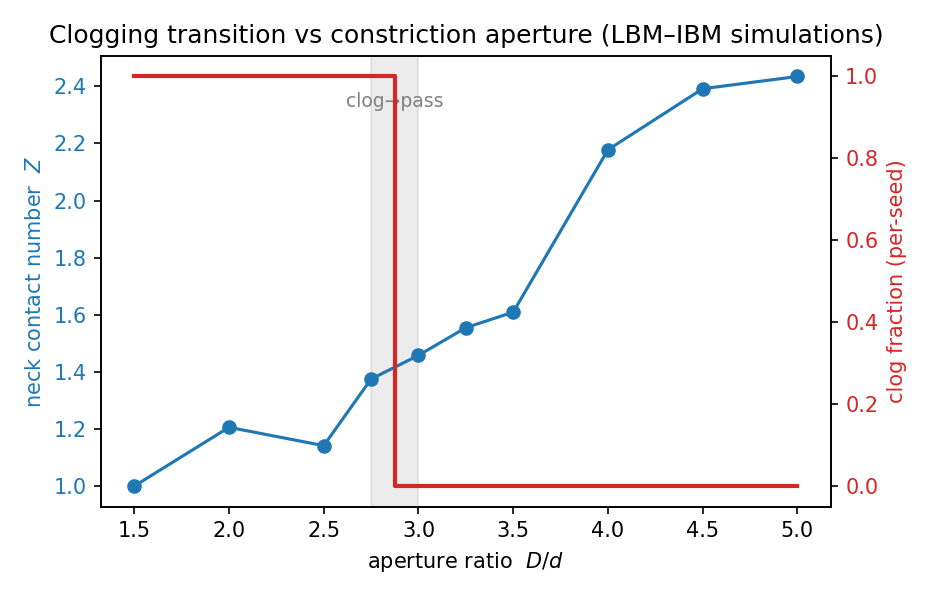
\includegraphics[width=0.78\linewidth]{fig1_phase.png}
\caption{Clogging transition versus constriction aperture from the
LBM--IBM runs. The neck contact number $Z$ (blue) grows with the
aperture ratio $D/d$, while the run-level clog fraction (red) drops from
one to zero between $D/d=2.75$ and $3.0$ (shaded), consistent with the
$D/d\approx 2$--$3$ arching threshold of the suspension-clogging
literature.}
\label{fig:phase}
\end{figure}

\subsection{Classifying configurations}
\label{sec:res-gnn}

Trained on the pooled frames, the network learns to separate clogging
from flowing configurations well. On the held-out frames it reaches an
accuracy of $0.78$, a balanced accuracy of $0.78$, and an area under the
ROC curve of $0.93$ (Figure~\ref{fig:gnn}). The ROC curve lies well above
the diagonal across the whole range of operating points, so the model
ranks clogging configurations above flowing ones reliably; the
class-weighted loss prevents it from defaulting to the majority class,
which is why the balanced accuracy tracks the raw accuracy despite the
$120{:}176$ class imbalance.

\begin{figure}[t]
\centering
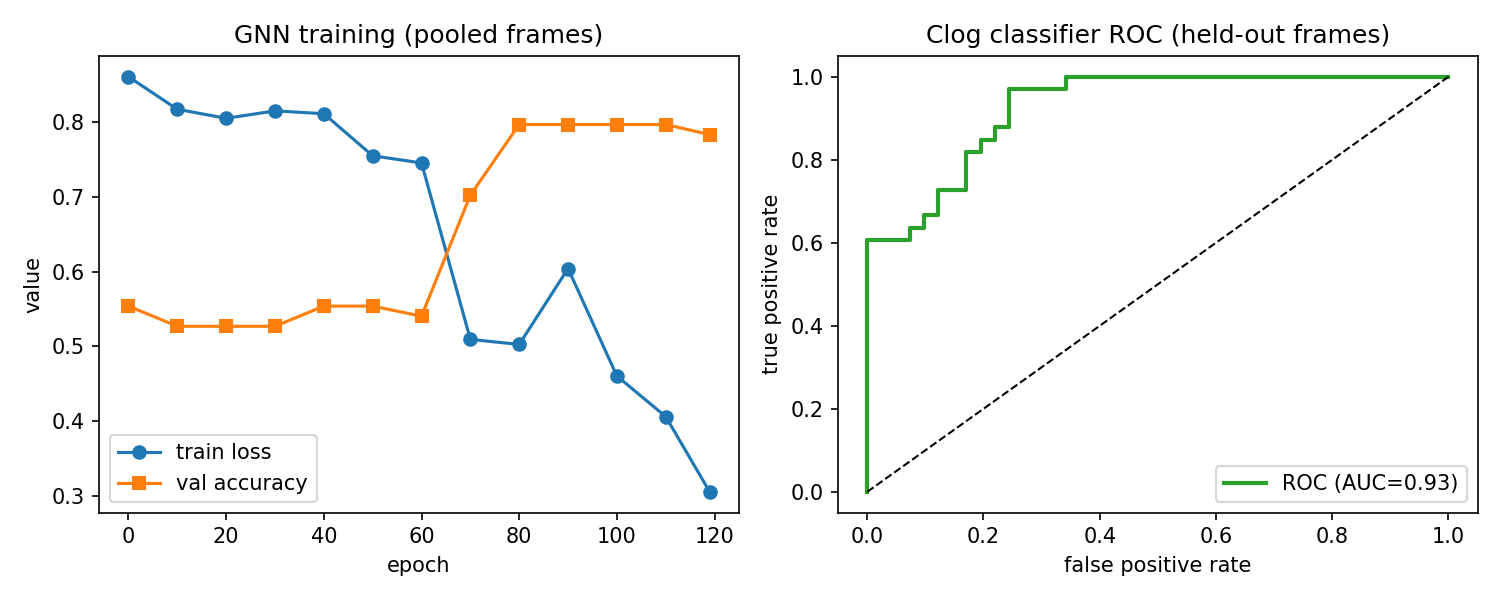
\includegraphics[width=\linewidth]{fig2_gnn_training.png}
\caption{Graph-classifier training and discrimination. \textbf{Left:}
training loss and validation accuracy over $120$ epochs on the pooled
frames. \textbf{Right:} ROC curve on held-out frames, with area under
the curve $0.93$; the dashed line is the chance diagonal.}
\label{fig:gnn}
\end{figure}

\subsection{Generalisation across runs}
\label{sec:res-loro}

The leave-one-run-out test is the more demanding and more informative
one. Figure~\ref{fig:loro} reports the per-aperture accuracy when each
run is removed from training in turn. The mean over the ten folds is
$0.87$: the network classifies the frames of an unseen aperture
correctly $87\%$ of the time on average, with $0.92$ on the flowing runs
and $0.79$ on the clogging runs. The accuracy is high and stable away
from the transition --- $0.97$--$1.00$ at the clear-clog apertures
$D/d\le 2.0$ and the clear-flow apertures $D/d\ge 4.0$ --- and collapses
at exactly one fold, $D/d=2.75$, where it reaches only $0.43$. That fold
is the last clogging aperture before the transition; when it is removed,
the training set contains clogging examples no closer than $D/d=2.5$ and
flowing examples no closer than $D/d=3.0$, so the network has seen
nothing at the boundary and is forced to extrapolate across it. The
failure is therefore localised exactly where the physical outcome is
itself most ambiguous, rather than being a systematic weakness of the
model.

\begin{figure}[t]
\centering
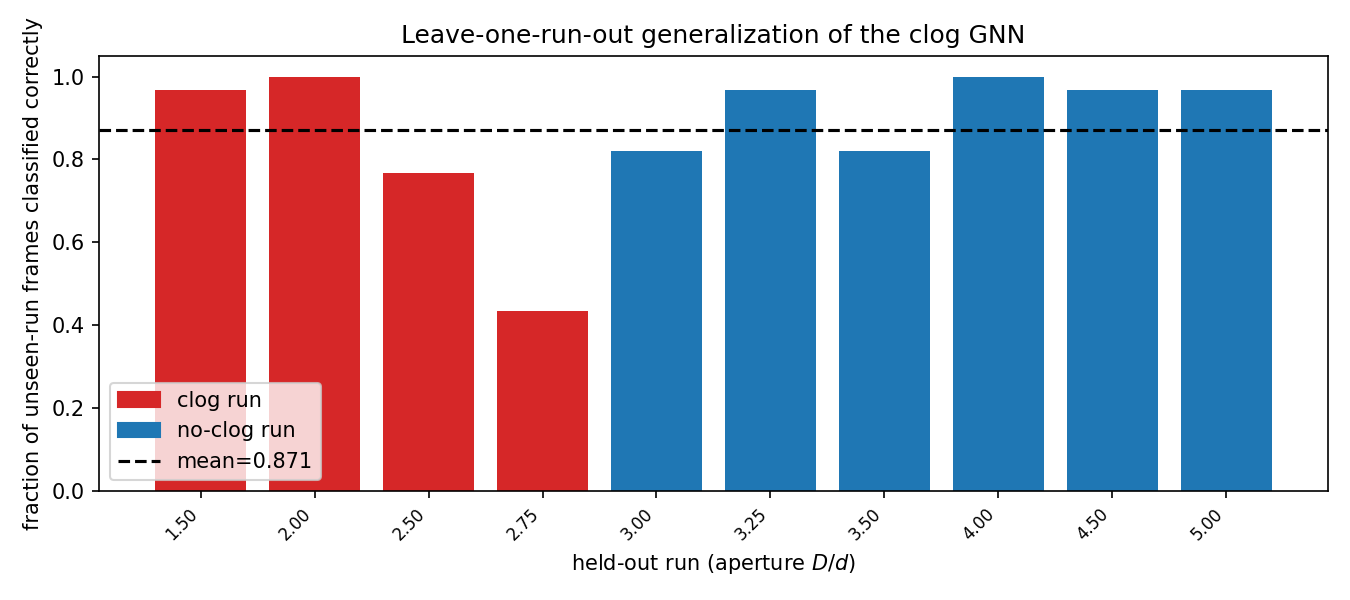
\includegraphics[width=\linewidth]{fig3_loro.png}
\caption{Leave-one-run-out generalisation. Each bar is the fraction of a
held-out aperture's frames classified correctly after retraining on the
other nine apertures; red bars are clogging runs, blue bars flowing
runs, and the dashed line is the mean ($0.87$). The model is strong away
from the transition and weak only at $D/d=2.75$, the aperture sitting on
the clog/flow boundary.}
\label{fig:loro}
\end{figure}

\subsection{Where the contacts concentrate}
\label{sec:res-graphs}

The two regimes are distinguished not by the overall density of the
contact network --- both are dense suspensions --- but by where in the
channel the contacts sit relative to the neck. Figure~\ref{fig:graphs}
averages each capsule's contact degree over its streamwise position,
pooled separately over all frames of the clogging and the flowing runs.
Upstream of the neck the two ensembles are similar, as expected for a
dense plug. At the constriction they part company. In the clogging
ensemble the contact degree collapses inside the throat and there are
essentially no capsules downstream of it: the narrow gap admits at most
a single capsule, and the rest of the suspension is held back by the
arch. In the flowing ensemble the contact degree stays elevated through
the throat and the profile extends well past it, because capsules are
continually carried through and populate the downstream channel. This
streamwise asymmetry --- a sharp loss of contacts and of downstream
occupancy at the neck --- is the structural fingerprint that the
classifier exploits, and it is made explicit to the network through the
node positions and the edge gap and approach-rate features.

\begin{figure}[t]
\centering
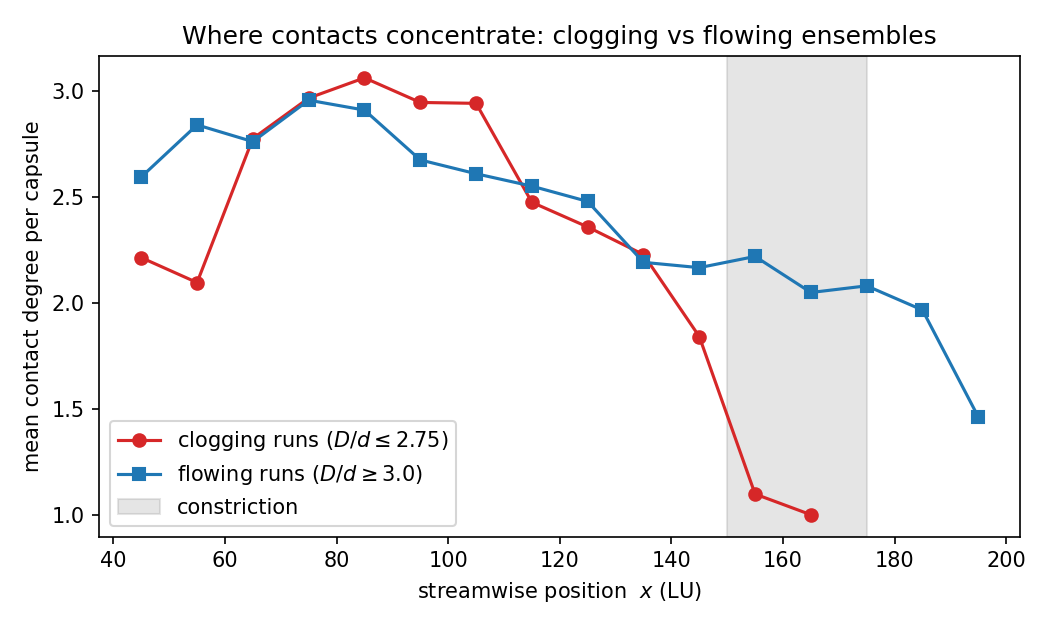
\includegraphics[width=0.74\linewidth]{fig4_graphs.png}
\caption{Mean contact degree per capsule as a function of streamwise
position, averaged over all frames of the clogging runs ($D/d\le 2.75$,
red) and the flowing runs ($D/d\ge 3.0$, blue); the shaded band is the
constriction. The two ensembles coincide upstream but diverge at the
neck: the clogging ensemble loses its contacts in the throat and has no
downstream occupancy (the arch admits at most one capsule), whereas the
flowing ensemble stays connected through the neck and extends
downstream.}
\label{fig:graphs}
\end{figure}

% ---------------------------------------------------------------------
\section{Discussion}
\label{sec:discussion}

The central finding is that a single static snapshot of the contact
network is enough to predict, with useful and transferable accuracy,
whether a soft-particle suspension is clogging. The network never sees
the dynamics; it is given only who is touching whom and the local
geometry of those contacts, and from that it recovers the collective
outcome. This supports a view of clogging as a property encoded in the
instantaneous force-bearing network --- the same picture that underlies
the statistical-mechanical description of jamming --- and it shows that
the encoding is learnable directly from configurations rather than
having to be summarised by hand-chosen order parameters.

Nothing in the method is specific to our capsules or to this geometry.
The network is handed only a generic contact graph --- particles as
nodes, contacts as edges, with a few local geometric features --- so the
same recipe should carry over with little change to other particulate
systems in which a collective state is written into the network of
contacts. Granular flow in silos and hoppers, colloidal fouling of
membranes and packed beds, and cell or capsule suspensions in confined
vessels are all natural candidates: in each case a structural snapshot
could be used to flag an incipient arch or jam, and more generally to
detect emergent network signatures that are awkward to capture with a
single hand-built order parameter.

The leave-one-run-out result is what gives the claim its weight. A
random split over frames would have reported a flattering number,
because frames from one simulation are highly correlated and a model can
recognise a run it has partly seen. By removing an entire aperture, the
LORO test asks the network to label configurations that are genuinely
new, and the $0.87$ mean shows that the contact-network signature it has
learned is not run-specific. The single weak fold at $D/d=2.75$ is
instructive rather than disappointing: it is the aperture exactly on the
transition, and once it is removed the boundary is unrepresented in
training. A classifier cannot be expected to place a sharp boundary it
has never observed, and the human-meaningful conclusion is the same one
the physics gives --- the outcome right at the transition is intrinsically
uncertain.

We also report a negative result that we think is useful. To strengthen
the boundary we tried augmenting the data with a second, jittered
realisation of each aperture, reasoning that a near-twin of the held-out
boundary run in the training set would help. It did the opposite: the
leave-one-run-out accuracy fell from $0.87$ to $0.70$. Near a sharp
transition the outcome is so sensitive to the microscopic arrangement
that two jittered realisations of the same nominal aperture can land on
opposite sides of the boundary, so the augmentation injected label noise
exactly where the model is most fragile. The lesson is that the binary
run-level label is the limiting resource near the transition, and that
more realisations do not help unless the label itself is made smoother;
a continuous target such as the escaped fraction, or a per-frame
``bridged'' label, would be the more promising route.

Several limitations bound the scope of these results. The model is
two-dimensional, so the arches are line-spanning rather than the
three-dimensional vaults of a physical silo or vessel; we expect the
qualitative contact-network signature to carry over, but the threshold
and the absolute accuracies will shift in three dimensions. We fixed the
capillary number, so deformability enters only through a single value
and not as a control variable; sweeping it would test whether the same
network generalises across softness as well as across geometry. The
clogging label is binary and assigned at the run level, which, as the
augmentation experiment showed, is the weakest point of the pipeline
near the transition. Finally, the data set is modest --- ten runs and a
few hundred graphs --- so the absolute numbers should be read as a
proof of principle rather than a converged benchmark. None of these
caveats undercuts the central result; they map out exactly what a larger
study would need to vary.

% ---------------------------------------------------------------------
\section{Conclusion}
\label{sec:conclusion}

We have shown that the clogging of a deformable-particle suspension at a
microfluidic constriction can be predicted from the instantaneous
contact network by an edge-aware graph neural network. A
two-dimensional lattice-Boltzmann immersed-boundary model, run across
ten aperture ratios, reproduces the expected arching threshold near
$D/d\approx 3$; converting each frame to a graph of capsules and
contacts and training a message-passing classifier yields an area under
the ROC curve of $0.93$ on held-out frames and, under a stringent
leave-one-run-out test, a mean accuracy of $0.87$ on apertures the
network has never seen, failing only at the single aperture on the
transition. The instantaneous contact network thus carries a learnable
and transferable signature of imminent clogging, and the work supplies a
reproducible route from a mesoscale physics solver to a graph-based
predictor. Natural extensions are to make the label continuous, to add
the capillary number as a second control parameter, to move to three
dimensions, and to use the trained network's attributions to read off
which contact-network features mark an incipient arch --- turning the
predictor into a tool for discovery as well as classification.

% ---------------------------------------------------------------------
\section*{Data and code availability}

The simulation engine, the graph-extraction and graph-neural-network
code, and the scripts that generate the data set, train the classifier,
run the leave-one-run-out evaluation and produce every figure in this
paper are available from the author on reasonable request. The bulk
trajectory output is regenerable from the provided scripts and fixed
random seeds.

\section*{Declaration of competing interest}

The author declares no competing interests.

% ---------------------------------------------------------------------
\bibliography{references}

\end{document}
